\section{Preliminaries and Our Main Theorem}
A (symmetric) constraint function
(a.k.a. signature) of arity $n$
is $f = [f_0, f_1, \ldots, f_n]$, where $f_i$ denotes the function
value  on inputs of Hamming weight $i$.
E.g., the  ternary \textsc{Exact-One} function
is  $[0,1,0,0]$, and
the ternary \textsc{Equality}
function $\left(=_{3} \right)$
is  $[1,0,0,1]$.
In this paper we consider the following 
%subclass 
set of $\operatorname{Holant}$ problems, denoted by 
$\plholant{f}{(=_3)}$,
where $f$ is a ternary function. An input is a signature grid $\Omega$ consisting of a planar 3-regular bipartite graph $G = (U,V,E)$, where each vertex in $U$ is assigned 
%a ternary symmetric constraint function
%(also called a signature) 
$f= [f_0,f_1,f_2,f_3]$ with values $f_i \in \mathbb{Q}$, and each vertex in $V$ is assigned $\left(=_{3} \right)$. The Holant problem
is to compute
%the constraint function \textsc{Equality} of arity 3, denoted by 
 
%%% since we deal with symmetric functions. no need for cyclic order
%The input $\Omega$ also specifies for every signature a cyclic order starting from some edge. The problem is to compute the quantity
$$
\operatorname{Holant}\left(\Omega\right) = \sum_{\sigma: E \rightarrow \{ 0,1\}} \prod_{u \in U} f\left(\sigma |_{E(u)}\right) \prod_{v \in V} \left( =_{3} \right) \left(\sigma |_{E(v)}\right).
$$

%Equivalently, this  can be stated as a  weighted counting constraint satisfaction problem on Boolean variables
%defined on planar 3-regular bipartite graphs:
%The input is a planar 3-regular  bipartite graph $G = (U,V,E)$,
%where  every $v \in V$ is a Boolean variable and
% every $u \in U$ represents the nonnegative valued constraint function $f$.
% An edge $(u,v) \in E$ indicates that $v$ appears in
% the constraint at $u$. Being 3-regular means that
% every constraint has 3 variables and every variable
% appears in 3 constraints.
%$\CSP\left( \{f\}\right)$ where $f$ is a function $f:\{0,1\}^3 \rightarrow \mathbb{R}_{\geq 0}$ mapping Boolean variables to the non-negative (algebraic) real numbers. 

For clarity, we shall call vertices in $U$ are on the left hand side (LHS) and vertices in $V$ are on the right hand side (RHS). 
%
%%% JYC: above you already used "arity"
%%% in intro already defiend symmmtric notation.
%The number of inputs for a signature is called its {\em arity}. A signature with one, two, or three inputs is called a {\em unary, binary} or {\em ternary} signature, respectively. A Boolean signature is called {\em symmetric} if its value only depends on the Hamming weight of the inputs. We adopt the compact notation $f = [f_0,f_1,f_2,f_3]$ to represent the ternary symmetric signature $f$ where $f\left(0,0,0\right) = f_0$, $f\left(0,0,1\right)=f\left(0,1,0\right) = f\left(1,0,0\right) = f_1$, $f\left(0,1,1\right)=f\left(1,0,1\right) = f\left(1,1,0\right) = f_2$ and $f\left( 1,1,1\right) = f_3$. The \textsc{Equality} of arities 3 is $\left(=_{3} \right) = [1,0,0,1]$. We can also regard a Boolean 
%%% we never do any non-Boolean domain in this paper. so no need to say
%%% boolean. it further confused with boolean valued signatures.
We can write a  signature of arity $n$ as a vector in 
%the space 
$\mathbb{Q}^{2^n}$ indexed in lexicographical order. 
%With this point of view, 
%A symmetric signature  of arity $n$ can be specified by $n+1$ values,
%$f = [f_0, f_1, \ldots, f_n]$, where $f_i$ denotes the function
%value  on inputs of Hamming weight $i$.
A 
(symmetric) 
signature $f$ is  {\em degenerate} if there exists a unary signature $u \in \mathbb{C}^2$ such that $f = u^{\otimes n}$, the $n$th tensor power.

The main result of this paper is the following dichotomy theorem:
\begin{theorem}\label{thm:main}
\plholant{f}{(=_3)} where $f = [f_0,f_1,f_2,f_3]$ and  $f_i \in \mathbb{Q}$ {\rm (}$0 \le i \le 3${\rm )} is \numP-hard except in the following cases, for which the problem is in $\operatorname{FP}$:
(1) $f$ is degenerate;
(2) $f = [a, 0, 0, b]$, for some $a, b$;
(3) $f = [a,0,\pm a,0], [0,a,0,\pm a], [a,-a,-a,a], [a,a,-a,-a]$ for some $a$;
(4) $f = [a, b, b, a]$ or $f =[a,b,-b,-a]$, for some $a, b$;
(5) $f= [3a+b,-a-b, -a+b, 3a-b]$ for some $a, b$.
Without the
planar restriction, the 
problem 
$\operatorname{Holant}(f\, |\,(=_3))$ remains in $\operatorname{FP}$ in cases (1), (2) and (3), but \#P-hard in cases
(4) and (5).
\end{theorem}
%\begin{theorem}\label{thm:main}
%\plholant{[f_0,f_1,f_2,f_3]}{(=_3)} where $f_i \geq 0$ {\rm (}$0 \le i \le %3${\rm )} is \numP-hard except in the following cases, for which the problem is %in $\operatorname{FP}$:
%(1) $[f_0,f_1,f_2,f_3]$ is degenerate;
%(2) $f_1=f_2=0$;
%(3) $[(f_0=f_2=0) \wedge (f_1=f_3)]$ or $[(f_1=f_3=0) \wedge (f_0=f_2)]$;
%(4) $(f_0=f_3) \wedge (f_1=f_2)$.
%\end{theorem}

In case (1), the signature $f$  decomposes into
three unary signatures. In case (2), $f$ is a generalized
equality. In  case (3), $f$ is in the affine class. In case (4), the Holant problem is transformable to planar \#PM with matchgates
(see more details about these tractable classes in~\cite{cai2017complexity}). In case (5), the planar P-time tractability is 
 \emph{neither} by  Valiant's holographic reduction alone,
  \emph{nor} entirely independent from it. Rather it is by a 
  combination of a holographic reduction together with
  a global argument. 

As mentioned in Section~\ref{sec:intro},
counting \texttt{Cubic-Planar-X3C} is just
\plholant{[0,1,0,0]}{(=_3)}, the counting problem of Moore and Robson~\cite{MooreR01}.
%Cubic Planar \textsc{Exact-3-Cover},
It clearly belongs to this class.
It is also equivalent to Cubic Planar Monotone 1-in-3 SAT. 
By Theorem~\ref{thm:main}, it is \#P-complete.
%settles this open problem: 

To see that case (5) is planar tractable,
we prove 
for any $a$ and $b$,
the value of \plholant{f}{(=_3)} for $f = [3a+b, -a-b, -a+b, 3a-b]$ on any planar signature grid exactly equals   the value of \plholant{[0,2a,0,0]}{[0,1,0,0]} on the same signature grid,
and thus can be computed by the FKT algorithm
for counting perfect matchings. Indeed, by a holographic transformation
using $H = \left[\begin{smallmatrix}1 & 1 \\ 1 & -1\end{smallmatrix}\right]$ we have the following sequence of equivalences:
%, we get the following equivalence by performing a holographic transformation:
\begin{eqnarray*}
   %\begin{split}
       \plholant{f}{(=_3)} & \equiv_{T} & \plholant{fH^{\otimes 3}}{(H^{-1})^{\otimes 3}(=_3)}\\  &  \equiv_{T} & \plholant{[0,0, 2a,2b]}{[1,0,1,0]}\\& \equiv_{T} & \plholant{[0,0,2a,0]}{[0,0,1,0]} \\  &\equiv_{T} & \plholant{[0,2a,0,0]}{[0,1,0,0]} 
    % \\&  \begin{cases} = 0\hfill  \text{if $a=0$} \\\equiv_{T}\holant{[0,1,0,0]}{[0,1,0,0]} \hfill  \text{else}
    %   \end{cases}
   %\end{split}
\end{eqnarray*}
where the third equivalence follows from the observation that for each nonzero
term in the Holant sum, every vertex on the LHS has at least two of three edges
assigned 1 (from $[0, 0, 2a, 2b]$), meanwhile every vertex on the RHS
has at most two of three edges assigned 1 (from $[1, 0, 1, 0]$). The graph being
bipartite and 3-regular, the number of vertices on both sides must equal, thus
every vertex has exactly two incident edges assigned 1. 


% MK3
  An example of a planar tractable
  problem that belongs to case (5) is as follows.
 It can be viewed as a covering problem on 3-uniform hypergraphs of degree 3.
We say  $(X, {\cal S})$  is a 3-regular $k$-uniform set system
(or 3-regular $k$-uniform hypergraph),
%$r$-regular $k$-uniform set system,
if ${\cal S}$ consists of a family of sets $S \subset X$ each of
size $|S| =k$, and every $x \in X$ is in exactly 3 sets.
%$r$ sets.
If $k=2$ this is just an ordinary 3-regular graph
(where the $2$-subsets are ordinary edges).  We consider
%$r$-regular graph.  We consider
 3-regular $3$-uniform set systems.
 We say ${\cal S'}$ is a \emph{leafless partial cover} 
 if every $x \in \bigcup_{S \in {\cal S'}} S$ belongs to more than
 one set $S  \in {\cal S'}$. We say $x$ is \emph{lightly covered}
 if $|\{S \in {\cal S'} : x \in S\}|$ is 2,
 and \emph{heavily covered} if this number is 3.
  
  \vspace{.1in}
\noindent$\mathbf{Problem:}$  \texttt{ Weighted-Leafless-Partial-Cover}.

\noindent$\mathbf{Input:}$ A 3-regular $3$-uniform set system
 $(X, {\cal S})$.

\noindent$\mathbf{Output:}$ $\sum_{\cal S'} (-1)^l 2^h$,
where the sum is over all leafless partial covers  ${\cal S'}$,
and $l$ (resp. $h$) is the number of $x \in X$ that are
{lightly covered} (resp. {heavily covered}).
  \vspace{.1in}

%One can show that 
Expressed in the Holant framework this problem is just
\holant{f}{(=_3)}, where $f = [1, 0, -1, 2]$.
This problem belngs to case (5)  with $a=1/2$ and $b= - 1/2$.

\begin{figure}[ht]
    \centering
    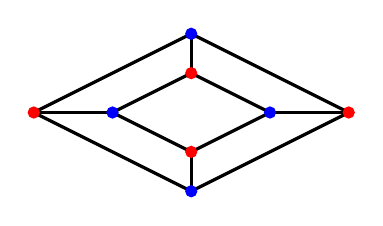
\begin{tikzpicture}[scale=0.5]
        \draw[very thick] (-4,0)--(0,2);
        \draw[very thick] (-4,0)--(-2,0);
        \draw[very thick] (-4,0)--(0,-2);

        \draw[very thick] (4,0)--(0,2);
        \draw[very thick] (4,0)--(2,0);
        \draw[very thick] (4,0)--(0,-2);

        \draw[very thick] (0,1)--(0,2);
        \draw[very thick] (0,1)--(2,0);
        \draw[very thick] (0,1)--(-2,0);

        \draw[very thick] (0,-1)--(0,-2);
        \draw[very thick] (0,-1)--(2,0);
        \draw[very thick] (0,-1)--(-2,0);
        
        \filldraw [blue] (0,2) circle (4pt);
        \filldraw [blue] (0,-2) circle (4pt);
        \filldraw [blue] (2,0) circle (4pt);
        \filldraw [blue] (-2,0) circle (4pt);
        
        \filldraw [red] (-4,0) circle (4pt);
        \filldraw [red] (4,0) circle (4pt);
        \filldraw [red] (0,-1) circle (4pt);
        \filldraw [red] (0,1) circle (4pt);
    \end{tikzpicture}
    \caption{A small instance for the problem \texttt{Weighted-Leafless-Partial-Cover}}
    \label{problem example}
\end{figure}

Figure~\ref{problem example} illustrates a small instance of this problem. Blue dots represent elements $x$ and red dots represent the family of sets $S$. An element $x$ is contained in a set $S$ if and only if the blue dot for $x$ is connected to the red dot for $S$. It is not hard to see that there are exactly 6 leafless partial covers, which are $\emptyset$, any family of 3 sets (there are 4 of them), and the family of all 4 sets. Therefore, the Holant value of this instance is $1 + 4(-1)^32^1+2^4 = 9$. 
One can also verify that there are 
exactly 9 distinct perfect matchings in the graph
in Figure~\ref{problem example}.


Therefore, it is known that cases (1)--(5) are
in $\operatorname{FP}$. The main claim lies in that all other cases are \numP-hard over planar graphs.
The cases (4) and (5) capture precisely those problems
that are \#P-hard on general but in FP on planar graphs; neither case alone does that.
% When proving our main result, we shall apply the following dichotomy theorem on 2-3 planar Holant problems~\cite{KowalczykC16}:

% \begin{theorem}\label{thm:previous}
% Suppose $a,b \in \mathbb{C}$, and let $X = ab$, $Y = a^3+b^3$. Then \plholant{[a,1,b]}{(=_3)} is \numP-hard except in the following cases, for which the problem is in $\operatorname{FP}$:
% (1) $X=1$;
% (2) $X=Y=0$;
% (3) $X=-1$ and $Y=0$;
% (4) $X=-1$ and $Y^2=-4$; and
% (5) $4X^3=Y^2$.
% \end{theorem}

% We note that the case (5) $4X^3=Y^2$ in Theorem~\ref{thm:previous} is the only class of problems which are tractable over planar graphs but \numP-hard in general for \plholant{[a,1,b]}{(=_3)}. Its tractability is given by holographic transformation to the FKT algorithm.


%%%%%%%%%%%JYC 2/9/2023 I edited till here
%%%%%%%%%%%% now 11 pm
%%%%%%%%%%%
%%%%%%%%%%%

A gadget in this paper, such as those illustrated in Figure~\ref{f1} and Figure~\ref{a nice gadget},
is a planar 3-regular bipartite graph $G = (U, V, E_{\rm in}, E_{\rm out})$ with
internal edges $E_{\rm in}$ and dangling edges $E_{\rm out}$.
There can be $m$ dangling edges internally incident
to vertices from $U$ and $n$ dangling edges internally incident
to vertices from $V$. These $m+n$ dangling edges 
correspond to Boolean variables $x_1, \ldots, x_m, y_1, \ldots,  y_n$
and the gadget defines
a signature
\[f(x_1, \ldots, x_m, y_1, \ldots,  y_n)
=
\sum_{\sigma: E_{\rm in} \rightarrow \{ 0,1\}} \prod_{u \in U} f\left(\widehat{\sigma} |_{E(u)}\right) \prod_{v \in V} \left( =_{3} \right) \left(\widehat{\sigma}  |_{E(v)}\right),
\]
where $\widehat{\sigma} $ denotes the extension
of $\sigma$ by the assignment on the  dangling edges.
The variables $x_1, \ldots, x_m$ (respectively, $y_1, \ldots,  y_n$) are called 
LHS (respectively, RHS) variables and are to be connected 
externally to RHS (respectively, LHS) signatures
in $\plholant{f}{(=_3)}$.

%%% jyc the following para can be omitted in 10-page version
%To preserve the bipartite structure, we must be careful
%with any gadget construction in how each  external wire is
%to be connected.
%A LHS variable is internally connected in the gadget to a 
%signature on the LHS and must be externally  connected to a RHS signature.
%Conversely, a RHS variable is internally connected in the %gadget to a 
%signature on the RHS and must be externally  connected to a LHS signature.

Gadgets that are constructible for \plholant{f}{(=_3)} is severely limited due to  planarity and bipartiteness.
%, and a curious number-theoretic constraint. 
Suppose $g$ is the signature
%constraint
%function  
of a gadget construction with all of its variables  on the LHS.
%in~\cite{FanC21} 
Then by a simple counting argument, the arity of $g$ must be a multiple of 3.
The same is true for a  gadget construction
with all of its variables  on the RHS.
In particular, one cannot hope to produce any unary or binary signature on either side. However, being able to have unary or binary signatures at hand has been proven to be very useful in studying Holant problems.

To tackle this difficulty,
%in~\cite{CaiFL21} we considered {\em straddled} gadgets, 
{\em straddled} gadgets were introduced~\cite{CaiFL21}
which have both LHS and RHS  variables. For example, the gadget $G_1$ in Figure~\ref{f1}, after we place $f$ 
on the square vertex and  $(=_3)$ 
on  the circle vertex, 
has one variable on the LHS (the dangling edge that connects to  a square)  and one variable on the RHS (the dangling edge that connects to  a circle).
We list the values of 
a signature $f$ in a {\em signature matrix} $M_f$ where the row(s) $R$ and column(s) $C$ correspond to assignments,
\newcommand{\cupdot}{\mathbin{\mathaccent\cdot\cup}}
in lexicographic order, of input variables $X = R \cupdot C$.
 We may identify $f$ with $M_f$. 
 When two signatures  $M_f$ and $M_g$
 are composed by merging the dangling edges
 of the column variables of $f$ with the row variables of $g$, 
 the signature matrix of the resulting signature is the matrix product $M_fM_g$.
 %in such a way that respect bipartiteness,
% the signature matrices are multiplied.  
 %the
%representation of their signature matrices, the resulting signature can be computed as the matrix multiplication.
In our paper, the composition must respect the bipartiteness and planarity. Also, note that if a straddled gadget has $m$ dangling edges to be connected to RHS and $n$ dangling edges to be connected to LHS, then $m-n \equiv 0 \bmod 3$.
%We adopt the notation for the \emph{signature matrix} of
%a straddled signature that the row indices correspond to inputs for LHS variables and column indices  correspond to inputs for RHS variables. For example, the signature matrix for $G_1$ in Figure~\ref{some gadgets G_1} will be $\left( \begin{smallmatrix} f_0 &f_2 \\ f_1 &f_3\end{smallmatrix}\right)$. A binary straddled signature will be called {\em degenerate} if its signature matrix is of rank 1.

One crucial
%instrumental 
idea in~\cite{CaiFL21} is to interpolate \emph{degenerate} straddled binary signatures and use them as two unary signatures;
one of which is desired and the other is to be grouped together  to form an easily computable positive constant, which does not affect the complexity. 
%To  interpolate a signature $h$ from other given signatures means that
%there is a reduction from any instance $I$ where $h$ occurs,
%to polynomially many instances $\{I_s\}$ where $h$ does not occur,
%and from the Holant values of these polynomially many $\{I_s\}$ 
% we can compute the Holant value of $I$ in polynomial time. 
%
%
%We now recall the proof strategy in~\cite{FanC21} and motivate the study of Planar 3-way Edge Matching (P3EM). There, constrained by the limited number of gadgets that one could possibly construct in 3-regular bipartite Holant problems, we interpolate degenerate straddled binary signatures and connect them to $f$ on LHS. We then use up all other ends by connecting to $=_3$ on RHS. Since the straddled signature is degenerate, this will create an easily computable non-zero factor and yields a reduction from 2-3 regular bipartite Holant problems. 
However, the ``grouped together'' process destroys the planar structure and thus the reduction  fails  for planar graphs. However,
we can make it work  for planar graphs  if we can group
these leftover unaries three at a time within each face. 
This is where planar 3-way edge matching (P3EM) comes in.
Our theorem on P3EM will allow us to do that.
%assign for each degenerate straddled binary signature one of the two adjacent faces so that every face 
%gets assigned a multiple of 3 times. Starting from a 2-3 regular bipartite plane graph $G'$, if we consider it as the edge-vertex incidence graph of a 3-regular plane graph $G$, then the previous requirement is equivalent to assign each edge in $G$ to one of its two adjacent faces so that every face gets $0 \pmod{3}$ edge(s) assigned.

More formally, let $G = (V, E)$ be an undirected plane graph, i.e., a planar graph
with a given planar embedding. We allow $G$ to be a multi-graph, i.e.,
parallel edges  and self-loops are allowed. A planar 
3-way edge matching (P3EM) is a partition of $E$ into a collection $M$
of 3-edge subsets $E = \bigcup_{t \in M} t$ such that we can
add one vertex $v_t$ for each $t \in M$ and connect $v_t$ to
the three edges of $E$ in $t$ so that the resulting graph is
still a plane graph. In Section~\ref{section:P3EM}, we prove that a P3EM always exists for any plane 3-regular graph (except for some trivial cases) and, moreover, can be constructed in polynomial time. An often-used technique in dealing with plane graphs is first taking a spanning tree of the dual graph and picking a root node, e.g., the node associated to the outer face. Starting from a leaf, one argues that some invariant property can be ``propagated'' through the tree until finally reaching the root. This technique is used in~\cite{MooreR01} as well as in the proof of previous dichotomies concerning planarity~\cite{CaiF17, CaiFGW22}. However, this technique does not work in this case. New techniques have to be invented.
The proof of our P3EM theorem is a mixture of algebra and combinatorics, and it should be of independent interest.





%We remark that Theorem~\ref{thm:P3EM} has an interesting connection to the famous four color theorem. Tait showed that a bridgeless 3-regular plane graph can be face-colored with 4 colors if and only if it can be edge-colored with 3 colors. Note that the dual graph of any 3-regular plane graph is a triangulated graph, and the existence of the 3-edge-coloring in the original graph translates precisely to the existence of a way to assign each edge to one of three distinct colors in its dual graph so that the edges of every face are colored differently. Our result translates to the existence of a way to assign each edge to its adjacent vertices in its dual graph so that every vertex is assigned $0 \pmod{3}$ edges.

%Among other hardness results, we highlight the following theorem.


%The problem $\plholant{[0,1,0,0]}{(=_3)}$ is the counting version of what is called Cubic Planar Monotone 1-in-3 Satisfiability in~\cite{MooreR01} where it was shown to be $\operatorname{NP}$-hard. There, Moore and Robson showed the $\operatorname{NP}$-hardness through a chain of reductions using complicated gadgets and were not able to conclude the \numP-hardness of its counting version. By showing the problem $\plholant{[0,1,0,0]}{(=_3)}$ is \numP-hard, we answer one of their open questions in a affirmative case: the counting problem right tromino on the square lattice, or for the domino and straight tromino on the cubic lattice, is \numP-complete. Besides, our proof in fact gives a parsimonious reduction between $\plholant{[0,1,0,0], [0,1,0]}{(=_3)}$ and $\plholant{[0,1,0,0]}{(=_3)}$. The former problem is shown to be $\operatorname{NP}$-hard in~\cite{DyerF86}. Thus, our proof yields an arguably much simpler proof for the hardness of the decision problem. Last but not the least, as pointed out in~\cite{MooreR01}, problem $\plholant{[0,1,0,0]}{(=_3)}$ can also be viewed as the problem of counting the number of solutions to Exact Cover by 3-Sets where the associated hypergraph is 3-regular, 3-uniform and planar.

%The problem $\plholant{[0,1,0,0]}{(=_3)}$ has been open for more than twenty years. The main technique used in our proof is gadget construction, which has been widely used in Holant theory. We emphasize that there is a fundamental difference of gadget construction in terms of signatures and those of combinatorics. The former operates algebraically without demanding canonical one-to-one correspondence, unlike the latter.